\documentclass[11pt, letterpaper]{article}
\input{../../homework.tex}
\usepackage{titlepageBU}
\title{Problem Set 5}
\courseID{PY 355}
\courseSection{A1}
\begin{document}
\makeproblem
\section*{Problem 1}
Let $\vec{r}_a,\vec{r} _b$ be positions of galaxies $A,B$ relative to earth. Hubble's law states that
\[
	\vec{v} _a=H_0 \vec{r} _a,\qquad \vec{v} _b = H_0 \vec{r}_b
.\]
The position of galaxy $A$ relative to $B$ is given by $\vec{r} =\vec{r}_b-\vec{r} _a$. Similarly, the velocity of galaxy $A$ relative to $B$ is given by $\vec{v} =\vec{v}\vec{_b-v} _a$. It follows that
\[
	\vec{v} =\vec{v}_a - \vec{v}_b = H_0 \vec{r}_a - H_0 \vec{r} _b = H_0\left( \vec{r} _a - \vec{r} _b \right) =H_0 \vec{r} 
.\]
Therefore, Hubble's law is obeyed.
\section*{Problem 2}
\begin{figure}[ht]
	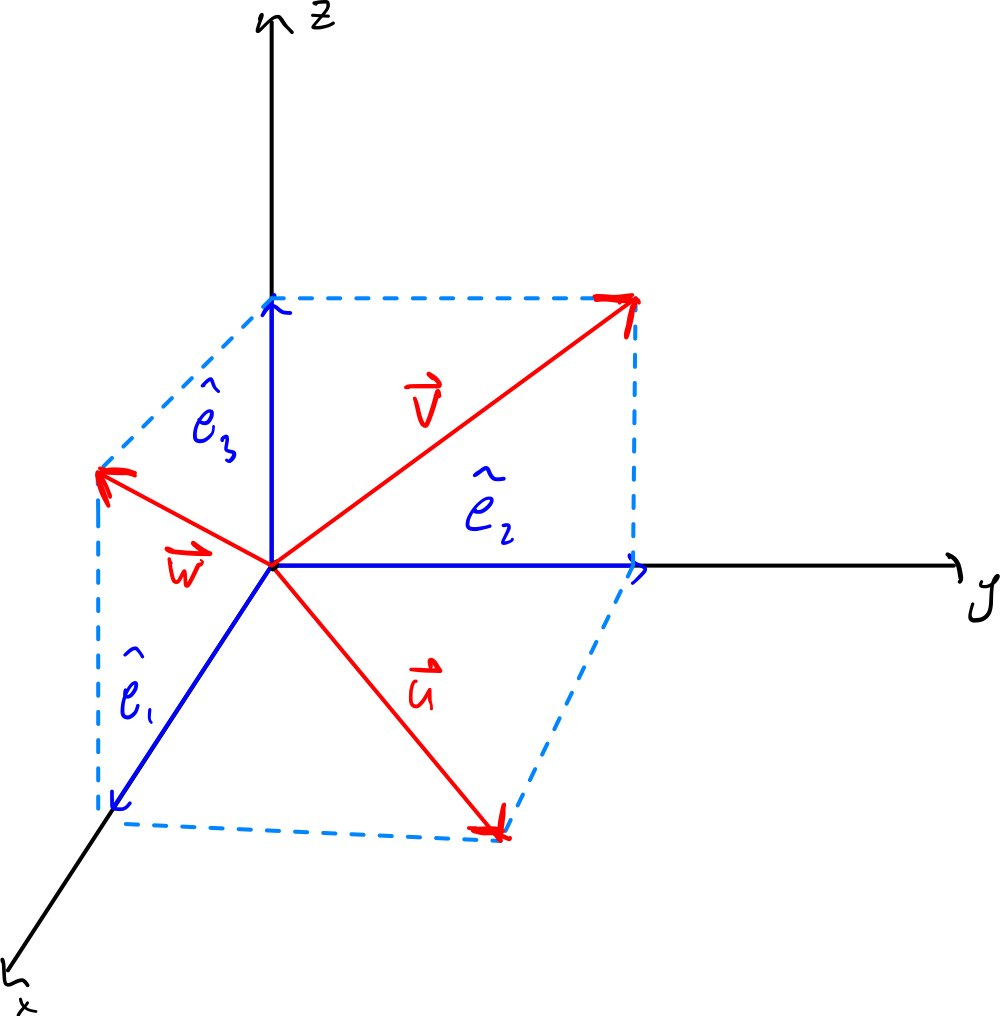
\includegraphics[scale=0.3]{../figures/image8.jpg}
	\centering
\end{figure}
\begin{itemize}
	\item Note that
		\[
			\vec{u} =\hat{e}_1 + \hat{e} _2 = \begin{pmatrix}
			1 \\
			1 \\
			0
			\end{pmatrix}
		.\]
		Thus,
		\[
			\left\| \vec{u}  \right\| =\sqrt{\begin{pmatrix}
			1 & 1 & 0
			\end{pmatrix}\begin{pmatrix}
			1 \\
			1 \\
			0
			\end{pmatrix}} =\sqrt{2} 
		.\]
		It should be extremely obvious that all vectors have the same length, so they all have length $\sqrt{2} $. This can be justified by noting that permutations of the order of basis elements are vector space isomorphisms, and any vector which is the sum of two elements of an orthonormal basis can be represented of the form $(1,1,0)$ in some permutation of some basis.
	\item It should also be obvious that they all are the same angle away from each other. Note that
		\[
			\theta =\arccos \left( \frac{\braket{\vec{u} }{\vec{v}}  }{\left\| \vec{u}  \right\| \left\| \vec{v}  \right\| }  \right) =\arccos \left( \frac{\begin{pmatrix}
			1 & 1 & 0
			\end{pmatrix}\begin{pmatrix}
			0 \\
			1 \\
			1
			\end{pmatrix}}{\sqrt{2} ^2}  \right) =\arccos \left( \frac{1}{2}  \right) =\frac{\pi }{3} 
		.\]
		Since all of their inner products are obviously 1, this is the angle between all of them.
	\item 
		\[
			\left( \vec{u} \times \vec{v}  \right) \cdot \vec{w} =\left( \left( \hat{e} _1 \times \hat{e} _2 \right) +\left( \hat{e} _1 \times \hat{e} _3 \right) +\left( \hat{e} _2 \times \hat{e} _2 \right) +\left( \hat{e} _2 \times \hat{e} _3 \right)  \right) \cdot \vec{w} =\left( \hat{e}_3 - \hat{e}_2 + \hat{e}_1 \right) \cdot \vec{w} 
		.\]
		\[
			\begin{pmatrix}
			1 & -1 & 1
			\end{pmatrix}\begin{pmatrix}
			1 \\
			0 \\
			1
			\end{pmatrix}=2
		.\]
		Therefore, it has a volume of 2 units.
\end{itemize}

\section*{Problem 3}
$\alpha	=1$ satisfies this equation. Note that
\[
	\vec{u} - \vec{t}  =\hat{e} _1 + \hat{e} _2 - \hat{e} _1 - \hat{e}_2 - \hat{e}_3=-\hat{e} _3,
\]
\[
	\vec{v} - \vec{t} =\hat{e} _2 + \hat{e} _3 - \hat{e} _1 - \hat{e} _2 - \hat{e} _3 = - \hat{e} _1
,\]
\[
	\vec{w} - \vec{t} = \hat{e} _3 + \hat{e} _1 - \hat{e} _1 - \hat{e} _2 - \hat{e} _3 = -\hat{e} _2
.\]
Since $\left\{ e_1,e_2,e_3 \right\} $ form an orthonormal basis, we have
\[
	\braket{- \hat{e} _1}{-\hat{e} _2} =-\braket{\hat{e} _1}{-\hat{e} _2} =\braket{\hat{e} _1}{\hat{e} _2} =0
,\]
\[
	\braket{- \hat{e} _2}{- \hat{e} _3} =- \braket{\hat{e} _2}{- \hat{e} _3} =\braket{\hat{e} _2}{\hat{e} _3} =0
,\]
\[
	\braket{- \hat{e} _3}{- \hat{e} _1} =-\braket{\hat{e} _3}{- \hat{e} _1} =\braket{\hat{e} _3}{\hat{e} _1} =0
.\]
\section*{Problem 4}
\begin{itemize}
	\item I have no idea if we've covered this in class, but a set of real-valued vectors is orthonormal if and only if the matrix $O$ formed by their rows is orthogonal; that is, $OO^T=1$. I will verify this computationally. Moreover, this implies that $O$ has an inverse, and thus is a bijection, and thus the span of the set of vectors is the entire space, and thus it will form a basis.
		\[
			\begin{pmatrix}
			1/\sqrt{3}  & 1/\sqrt{2}  & 1/\sqrt{6}  \\
			1/\sqrt{3}  & -1/\sqrt{2}  & 1/\sqrt{6}  \\
			1/\sqrt{3}  & 0 & -2/\sqrt{6} 
			\end{pmatrix}\begin{pmatrix}
			1/\sqrt{3}  & 1/\sqrt{3}  & 1/\sqrt{3}  \\
			1/\sqrt{2}  & -1/\sqrt{2}  & 0  \\
			1/\sqrt{6}  & 1/\sqrt{6}  & -2/\sqrt{6} 
			\end{pmatrix}
		\]
		\[
			=\begin{pmatrix}
			\frac{1}{3} +\frac{1}{2} +\frac{1}{6}  & \frac{1}{3} -\frac{1}{2} +\frac{1}{6}  & \frac{1}{3} -\frac{2}{6}  \\
			\frac{1}{3} -\frac{1}{2} +\frac{1}{6}  & \frac{1}{3} +\frac{1}{2} +\frac{1}{6}  & \frac{1}{3} -\frac{2}{6}  \\
			\frac{1}{3} -\frac{2}{6}  & \frac{1}{3} -\frac{2}{6}  & \frac{1}{3} +\frac{4}{6} 
			\end{pmatrix}=\begin{pmatrix}
			1 & 0 & 0 \\
			0 & 1 & 0 \\
			0 & 0 & 1
			\end{pmatrix}=1
		.\]
		Therefore, $O$ is orthogonal, and the vectors form an orthonormal set which spans $\mathbb{R} ^3$.
	\item We want to find a vector $\vec{c} =(c_1,c_2,c_3)$ such that
		\[
			c_1 \vec{e}_1 + c_2 \vec{e} _2 + c_3 \vec{e} _3= \vec{w} 
		.\]
		This is equivalent to asking that $O \vec{c} =\vec{w} $. Since $O$ is invertible, and $O^{-1} =O^T$, we have that $\vec{c} =O^T \vec{w} $. Computing this gives us
		\[
\begin{pmatrix}
			1/\sqrt{3}  & 1/\sqrt{3}  & 1/\sqrt{3}  \\
			1/\sqrt{2}  & -1/\sqrt{2}  & 0  \\
			1/\sqrt{6}  & 1/\sqrt{6}  & -2/\sqrt{6} 
			\end{pmatrix} \begin{pmatrix}
			1 \\
			0 \\
			0
			\end{pmatrix}=\begin{pmatrix}
			1/\sqrt{3}  \\
			1/\sqrt{2}  \\
			1/\sqrt{6} 
			\end{pmatrix}
		.\]
		Therefore,
		\[
			\vec{w} = \frac{1}{\sqrt{3} } \vec{e}_1 + \frac{1}{\sqrt{2} } \vec{e}_2 + \frac{1}{\sqrt{6} } \vec{e}_3
		.\]
		We can also verify this explicitly:
		\[
			\frac{1}{3} \begin{pmatrix}
			1 \\
			1 \\
			1
			\end{pmatrix}+\frac{1}{2} \begin{pmatrix}
			1 \\
			-1 \\
			0
			\end{pmatrix}+\frac{1}{6} \begin{pmatrix}
			1 \\
			1 \\
			-2
			\end{pmatrix}=\begin{pmatrix}
			1/3+1/2+1/6 \\
			1/3-1/2+1/6 \\
			1/3-2/6
			\end{pmatrix}=\begin{pmatrix}
			1 \\
			0 \\
			0
			\end{pmatrix}
		.\]
\end{itemize}
\section*{Problem 5}
\begin{itemize}
	\item We have
		\[
			\frac{\partial }{\partial x} \frac{1}{\sqrt{x^2+y^2+z^2} } =\frac{-x}{\left( \sqrt{x^2+y^2+z^2}  \right) } =-\frac{x}{r^3} 
		.\]
		The computation of the partial derivatives for the other two variables is the same. Therefore,
		\[
			\nabla f=\begin{pmatrix}
			-xr^{-3}  \\
			-yr^{-3}  \\
			-zr^{-3} 
			\end{pmatrix}=-\frac{1}{r^3} \begin{pmatrix}
			x \\
			y \\
			z
			\end{pmatrix}
		.\]
	\item $r^2=x^2+y^2+z^2$. The partial derivatives are all obviously 2 times the respective variable. Therefore,
		\[
			\nabla g=\begin{pmatrix}
			2x \\
			2y \\
			2z
			\end{pmatrix}
		.\]
	\item All of the partials are computed the same way, but with the respective variables switched. For this reason, I will only show one. Note that
		\[
			\frac{\partial }{\partial x} \sqrt{x^2+y^2+z^2} =\frac{2x}{x^2+y^2+z^2} =\frac{2x}{r} 
		.\]
		It follows that 
		\[
			\frac{\partial }{\partial x} e^r(x+y+z)=e^r+\left( \frac{\partial }{\partial x} r \right) e^r(x+y+z)=e^r\left(1+\frac{2x}{r} (x+y+z)\right)
		.\]
		Therefore,
		\[
			\nabla h=e^r \left(\begin{pmatrix}
			1 \\
			1 \\
			1
			\end{pmatrix}+2\frac{x+y+z}{r} \begin{pmatrix}
			x \\
			y \\
			z
			\end{pmatrix}\right)
		.\]
	\item Note that $r(1,1,1)=\sqrt{3} $. It follows that
		\[
			\nabla f(1,1,1)=-\frac{1}{\sqrt{3}^3 } \begin{pmatrix}
			1 \\
			1 \\
			1
			\end{pmatrix}=-\frac{1}{3\sqrt{3} } \begin{pmatrix}
			1 \\
			1 \\
			1
			\end{pmatrix}
		.\]
		The norm of this is
		\[
			\sqrt{\left( \frac{1}{3\sqrt{3} }  \right)^2\left( 1+1+1 \right) }=\frac{1}{3\sqrt{3} } \sqrt{3} =\frac{1}{3} 
		.\]
\end{itemize}
\section*{Problem 6}
\begin{itemize}
	\item Note that
		\[
			\frac{\partial V}{\partial x} =2x+y+6,\qquad \frac{\partial V}{\partial y} =2y+x
		.\]
		Setting these equal to $0$, we have that $x=-2y$, and thus
		\[
			2(-2y)+y+6=-3y+6=0\implies y=2
		.\]
		It follows that $x=-4$. We also have
		\[
			\frac{\partial ^2V}{\partial x^2} =2,\qquad \frac{\partial ^2V}{\partial y^2} =1,\qquad \frac{\partial ^2V}{\partial x \partial y} =1
		.\]
		The hessian determinant at this point is thus
		\[
			\begin{vmatrix}
			2 & 1 \\
			1 & 2
			\end{vmatrix}=4-2=2
		.\]
		Since this is positive, $V(-4,2)$ attains a minimum at $(-4,2)$. The value of this minimum is
		\[
			V(-4,2)=16+4-8-24=-12
		.\]
	\item Using the partials as calculated earlier,
		\[
			\nabla E=-\begin{pmatrix}
			2x+y+6 \\
			2y+x
			\end{pmatrix}
		.\]
	\item We have
		\[
			\nabla E(-4,2)=\begin{pmatrix}
			2(-4)+2+6 \\
			2(2)-4
			\end{pmatrix}=\begin{pmatrix}
			-8+8 \\
			4-4
			\end{pmatrix}=0
		.\]
\end{itemize}

\section*{Problem 7}
This follows from the product rule. Note that the $i$th component of $\nabla (uv)$ is simply
\[
	\frac{\partial uv}{\partial x_i} =\frac{\partial }{\partial x_i} (uv)=u \frac{\partial }{\partial x_i} v+v \frac{\partial }{\partial x_i} u
.\]
Therefore, each component is of this form. We can separate the vectors at the $+$ and factor out the functions $u,v$ as constants to obtain $\nabla (uv)=u\nabla v+v\nabla u$.
\section*{Problem 8}
I will do this componentwise again. The $i$th component of $\nabla (aF+bG)$ is
\[
	\frac{\partial }{\partial x_i} \left( aF+bG \right) =a \frac{\partial }{\partial x_i} F+b \frac{\partial }{\partial x_i} 
,\]
because partials are linear. Since every component is of this form, we can factor out the $a,b$ and break the vectors apart at the $+$ to obtain
\[
	\nabla (aF+bG)=a\nabla F+b\nabla G
.\]
\end{document}
